
%%% Local Variables:
%%% mode: latex
%%% TeX-master: t
%%% End:

\section{Results and Usecases} \label{S:results}

We report on some of our use cases while focussing in particular on
the use of virtual machines and virtual clusters, as well as giving an
outlook of selected planned improvements based on lessons learned.

\subsection{Heterogeneous VM Management}

Over the last 2 years we have used Cloudmesh in a number of classes
and research projects to access clouds from a variety of sources. This
includes the management of classes with more than 70 users, but also
the support of individual researchers with the need to conduct
infrastructure experiments. Cloudmesh has been shown to be able to
access Chameleon Cloud, CloudLab, Cybera in Canada, HP cloud, Amazon
WS, Azure. Most recently we also showcased potential access to
Jetstream. One of the interesting benefits of this rich diversity is
that educational efforts can be targeted for a particular platform
while the interface to them for managing virtual machines is the same.
In our experience with classes and potential user this is
an advantage, as when the switch of a single variable (e.g., the
name of the cloud) a VM or VC can be created on
a different infrastructure reducing the load on the original
system. Hence, reliability can be increased without introducing
additional complex and divergent interfaces for the diverse set of
clouds. Future use cases will include class use of {\em Comet\/} VC
for a planned graduate course that can serve up to 140 new
applicants to the newly created data science program at Indiana
University. As we demonstrated with Cloudmesh Client we would also be
able to access other XSEDE resources such as Jetstream and Bridges
once they become available to us and offer programable interfaces that
we can integrate in Cloudmesh.

\subsection{OnDemand Hackathon Support}

In February 2016 SDSC hosted a hackathon \cite{caida} related to the activities of
CAIDA the Center for Applied Internet Data Analysis. ``CAIDA provides macroscopic insights into
Internet infrastructure, behavior, usage, and evolution, fosters a
collaborative environment in which data can be acquired, analyzed, and
(as appropriate) shared, improves the integrity of the field of
Internet science, and informs science, technology, and communications
public policies.''  The hackathons theme was live measurements and
monitoring of the global Internet routing system (BGP). A total of 90
attendees participated in the event representing a mix of Academia,
Industry and Institutions. {\em Comet\/} provided compute resources to
participants, including several virtualized nodes, that were essential
for the success of the event. Over 15,000 SUs were used during 24
hours of activities. The virtualized nodes were especially important
as they allowed CAIDA adminstrators to install a different OS and
application software stack than that which exists on {\em Comet\/}.

\subsection{Open Science Grid}

The Open Science Grid (OSG) \cite{osg} provides an integrated facility
to access compute resources through distributed high throughput
computing for researchers in the US. The resources are contributed by
the community and organized by OSG. Many projects are executed on OSG,
one of which is the Laser Interferometer Gravitational-Wave
Observatory (LIGO). LIGO is ``designed to open the field of
gravitational-wave astrophysics through the direct detection of
gravitational waves predicted by Einstein's General Theory of
Relativity'' \cite{ligo}.

{\em Comet\/} has delivered 700,000 SUs to LIGO via OSG since its
inception. Thus {\em Comet} contributed considerably to both
efforts, OSG and LIGO. In November 2015 OSG began operating a VC on
{\em Comet} and immediately began running calculations related to LIGO. The
integration within OSG has been conducted in two modes to demonstrate
its wide usability (see Figure \ref{F:osg}).

\begin{figure}[htb]
  \centering
    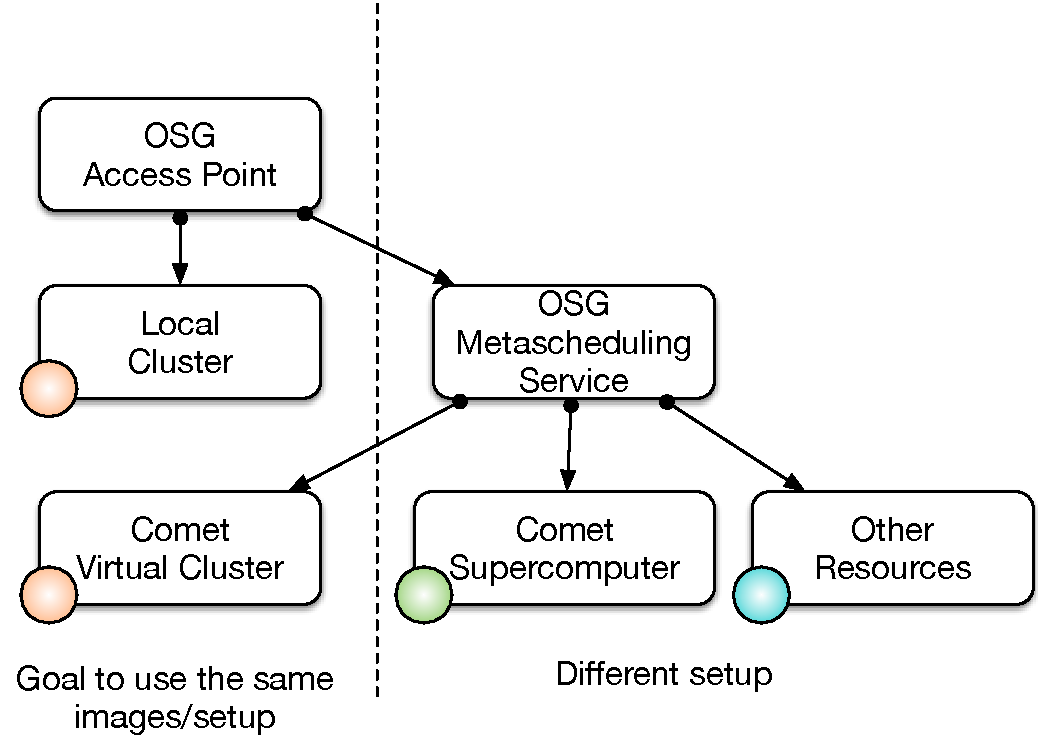
\includegraphics[width=1.0\columnwidth]{images/osg.pdf}
    \caption{Open Science Grid use cases}
    \label{F:osg}
\end{figure}

The first mode is the traditional integration of a supercomputing
allocation while utilizing the batch system and existing specialized
integration of batch job capabilities accessed by the OSG
metascheduler. This mode requires additional layers of abstraction
between the OSG metascheduler and the batch system on the compute
resource. The second one is the integration of a VC
that is based on software used for the operation of the local OSG
cluster and thus shares the same infrastructure requirements in
regards to operating system and other services. Hence no abstraction layer is
needed as a standard OSG system definition and software stack can be
used and run on the VC.  In contrast to other virtualization infrastructures and
efforts we are currently exploring the utilization of MPI jobs within
the VC to make use of the underlying high performance
networking infrastructure accessible from within the OSG VMs. These
VMs already utilize the virtualized InfiniBand HCAs to access storage.
